\documentclass{article}
\usepackage[utf8]{inputenc}
\usepackage[english,russian]{babel}
\usepackage{graphicx}
\usepackage{amsmath}
\DeclareGraphicsExtensions{.pdf,.png,.jpg}
\begin{document}
Постройте график функции
\begin{equation*}
y = 
 \begin{cases}
   x^2-4x+5 \text{, если } x \geq 1 \\
   x+1 \text{, если } x<1
 \end{cases}
\end{equation*}
и определите, при каких значениях $m$ прямая $y = m$ имеет с графиком ровно две общие точки.

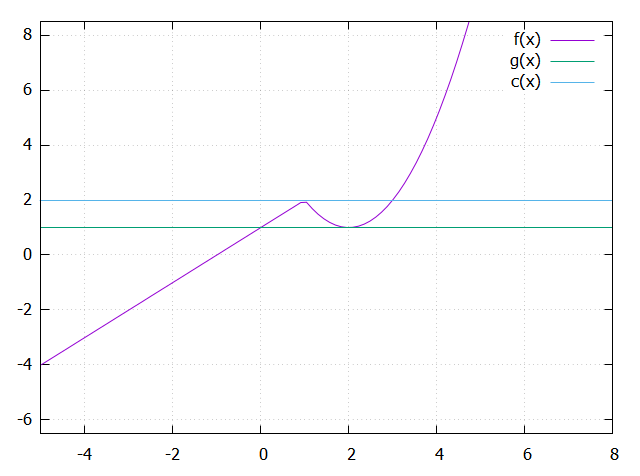
\includegraphics [scale=0.5]{plot.png}

1) $x=1$, $y=1+1=2$, т.е при $m=2$ ровно 2 общие точки.

2) $x^2-4x+5$,
$y_0 = \frac{-D}{4a}=1$, т.е при $m=1$ ровно 2 общие точки.

Ответ: При $m=1$, $m=2$
\end{document}